\documentclass{article}
\usepackage{amssymb}
\usepackage{amsmath}
\usepackage[utf8]{inputenc}
\usepackage[margin=1in]{geometry}
\usepackage{graphicx}
\usepackage{csquotes}

\linespread{1.2}

\usepackage{listings}
\lstset{
basicstyle=\small\ttfamily,
columns=flexible,
breaklines=true
}

\usepackage[
backend=biber,
style=alphabetic,
sorting=ynt
]{biblatex}

\addbibresource{bibliography.bib}

\newcommand\annotation[2]{\(\underbrace{\text{#1}}_\text{#2}\)}
\newcommand\topannotation[2]{\(\overbrace{\text{#1}}^\text{#2}\)}

\title{Summary: Computable Astronomical Diaries}
\author{Christopher Wolfram, Aaron Schein}
\date{November 2024}

\begin{document}

\maketitle

\section{Outline}

The Computable Astronomical Diaries project uses large language models (LLMs) to extract structured data from translations of ancient Babylonian astronomical texts. As an application of this dataset, we fit a statistical model to the data to estimate the sizes of units used by the Babylonians, and to estimate the times when they made observations.

\section{Background on the Astronomical Diaries}
The Astronomical Diaries are the product of the longest running data collection project in human history \autocite{steeleIntro, whoWrote}. Covering several hundred years from the mid 7th-century BCE to near the beginning of the first millennium, the diaries record daily astronomical observations (the positions of the Moon and planets relative to the fixed stars, times of eclipses, etc.), as well as observations of the weather, the level of the Euphrates river, prices of commodities in the market in Babylon, and more \autocite{sachsHunger}.

The Astronomical Diaries were written on clay tablets, several hundred of which have survived to the present. Many of these were transliterated, translated to English, and dated by Sachs and Hunger \autocite{sachsHunger}, and are now available online from Oracc (\url{https://oracc.museum.upenn.edu/adsd/}). However, researchers interested in the diaries still have to manually go through hundreds of pages of translations to extract the data they care about, which is often impractical.

\subsection{Example Text}
Below is an example excerpt of a translated Astronomical Diary:\footnote{-170E: \url{https://oracc.museum.upenn.edu/adsd/adart2/X201705}}

\begin{displayquote}
Year 141, kings Antiochus and Antiochus, his son. Month VII, the 1st (of which followed the 30th of the preceding month), sunset to moonset: 9°, measured. The 1st, the north wind blew. Night of the 2nd, the moon was 2 cubits behind $\alpha$ Scorpii. The 2nd, the north wind blew. Night of the 3rd, the moon was 2 1/2 cubits behind $\vartheta$ Ophiuchi. Night of the 6th, the moon was 4 cubits below $\beta$ Capricorni, the moon having passed 1/2 cubit to the east. Night of the 7th, the moon was 2 cubits in front of $\gamma$ Capricorni, the moon being 1 cubit low to the south. The 7th, Mercury's first appearance [in the east] in Libra, Mercury was 2/3 cubit behind Venus, [Mercury being ...] high to the north;
\end{displayquote}

\section{Parsing the Diaries}
There have been many papers and books published based on data from the Astronomical Diaries. However, they generally focus on a single slice of the data (such as all market quotations, planetary observations, etc.) Moreover, I am not aware of any that study the full bulk of lunar observations that make up a large fraction of the Diaries.

The goal of the Computable Astronomical Diaries project is to make the systematic data encoded in the Astronomical Diaries accessible in a computer-friendly format, making large-scale analysis of the entire corpus feasible.

Back in 2020, I created a format for representing observations in the Astronomical Diaries and an interface for inputting data into that format. After manually inputting data from a couple of texts, I calculated that it would take about 200 hours of work to curate the entire corpus. 200 hours is short enough to be possible, but long enough that I never did it (and as far as I know, nobody else has done it either).

However, LLMs are good at menial structured data extraction tasks and can process the entire Astronomical Diaries in a matter of minutes and at negligible cost.

We use GPT-4o from OpenAI to extract ``distance observations'' (such as ``the moon was 3 cubits in front of $\alpha$ Cancri'') from the Astronomical Diaries. We target distance observations because they make up the bulk of the diaries.

\subsection{Anatomy of a Distance Observation}
Here is an example of a distance observation:
\begin{displayquote}
\annotation{Night of the 9th}{day}, \annotation{last part of the night,}{time} \annotation{Mars}{object} was \annotation{1 cubit 8 fingers}{distance} \annotation{below}{relation} \annotation{$\eta$ Tauri}{reference}
\end{displayquote}
It gives the distance between an object (i.e. Mars) and a reference (i.e. $\eta$ Tauri) in a particular direction (i.e. ``below'').

\subsection{Prompting}
We use a multi-phase pipeline to extract observations.

The goal of the first phase is to identify which passages refer to which months. The translations provided by Sachs and Hunger include a month guide that indicates which sections of the translation correspond to which months \autocite{sachsHunger} (e.g. ``] II III [] V VI [''). The LLM is given this month guide along with the translation of the diary, and prompted to identify which months correspond to which line numbers in the translation.

In the second phase, observations are extracted by prompting the LLM to list observations in a text, along with the line numbers on which observations appear (allowing alignment with the first phase).

All prompts are available in the prompt appendix at the end of this document.

\subsection{Results}
There are a total of 7751 distance observations. The vast majority are lunar observations (6597).

\subsubsection{Example Data}
Below is a table showing extracted observations from the tablet AD -278B\footnote{X102702 on Oracc: \url{https://oracc.museum.upenn.edu/adsd/adart1/X102782}}:

\begin{figure}[h]
    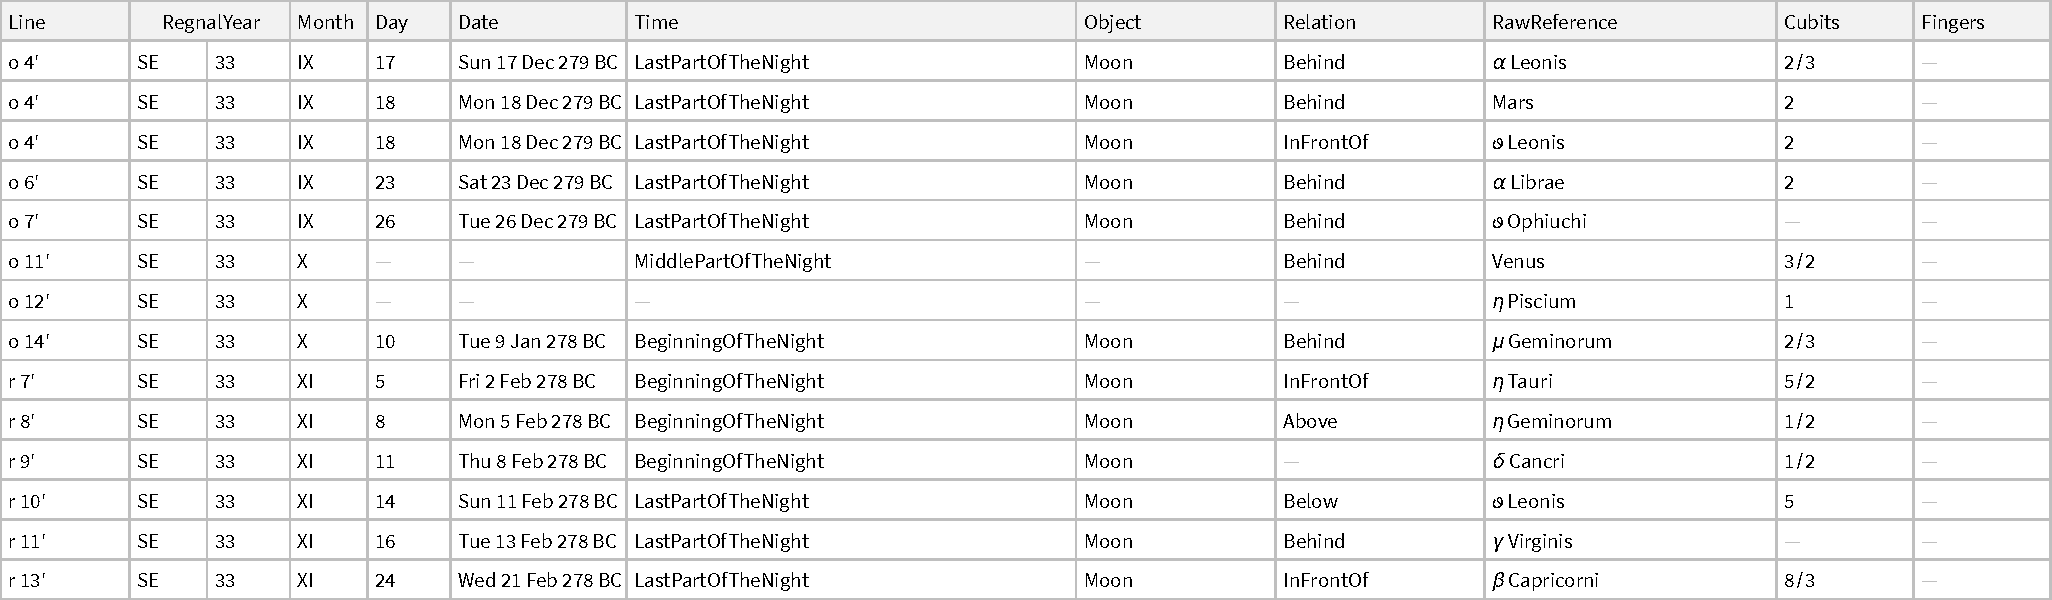
\includegraphics[width=1\linewidth]{X102782.pdf}
\end{figure}

This text is fairly typical in terms of the LLMs performance. Almost all observations were extracted correctly, with the only exception being a fragmentary observation on line r 7' that was missed.

% \subsubsection{Basic Properties}
% There are a total of 7892 distance observations. The vast majority are lunar observations (6711). Figure \ref{fig:objectFreqs} shows the number of observations of the planets.

% \begin{figure}[h]
%     \centering
%     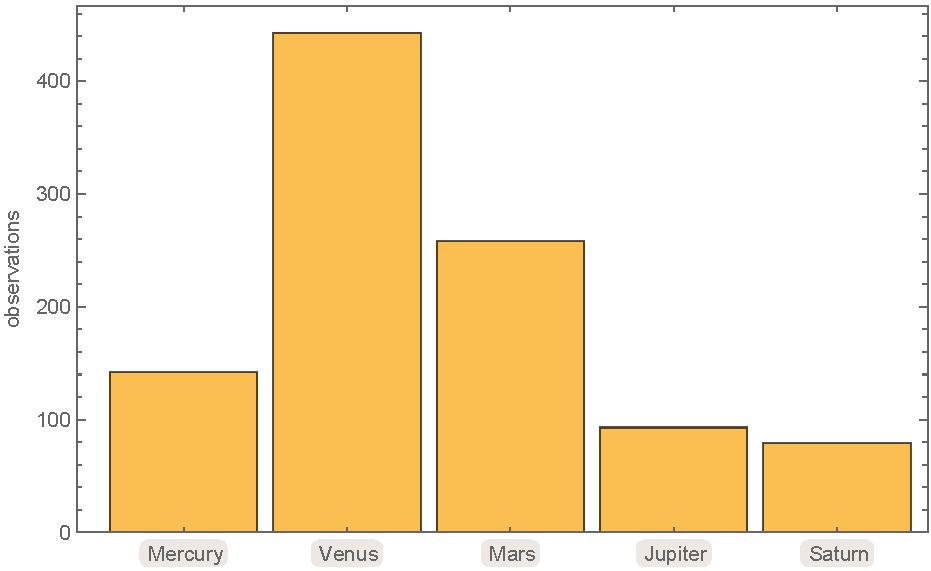
\includegraphics[width=0.6\linewidth]{objectFrequencies.pdf}
%     \caption{Number of observations for each planet.}
%     \label{fig:objectFreqs}
% \end{figure}

\subsubsection{Comparing to Modern Calculations}
Using the Parker and Dubberstein chronology \autocite{parkerDubberstein}, I computed Julian calendar dates for all of the observations (for which date information was not missing). Then, using JPL ephemerides, I computed the true positions of the referenced objects at midnight (UTC+3, the timezone of modern Iraq). The scatter plot in figure \ref{fig:scatter} shows the positions of observed objects relative to the reference objects (for example, the true position of the Moon relative to $\eta$ Geminorum).

\begin{figure}[h]
    \centering
    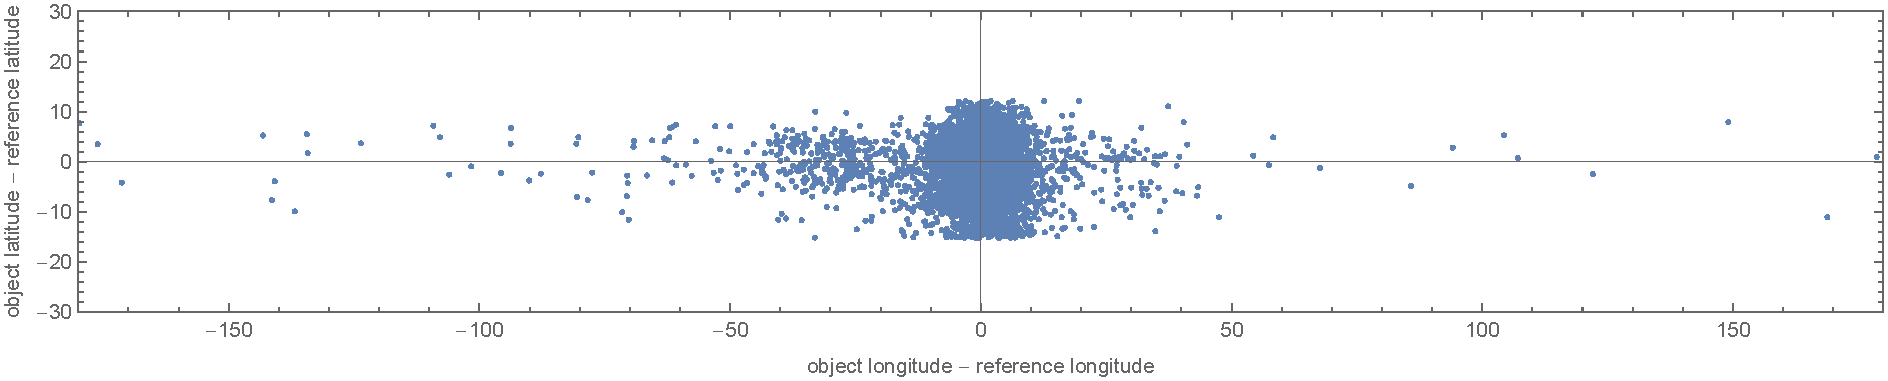
\includegraphics[width=\linewidth]{relativePositions.pdf}
    \caption{Relative positions of objects and references in the Astronomical Diaries, assuming observations were made at midnight UTC+3.}
    \label{fig:scatter}
\end{figure}

Next, I looked at only those observations where an object is said to be ``above'' or ``below'' a reference. Comparing to modern data, objects observed to be ``above'' a reference consistently have higher ecliptic latitude, while objects observed to be ``below'' has lower ecliptic latitude (figure \ref{fig:scatterAboveBelow}).

\begin{figure}[h]
    \centering
    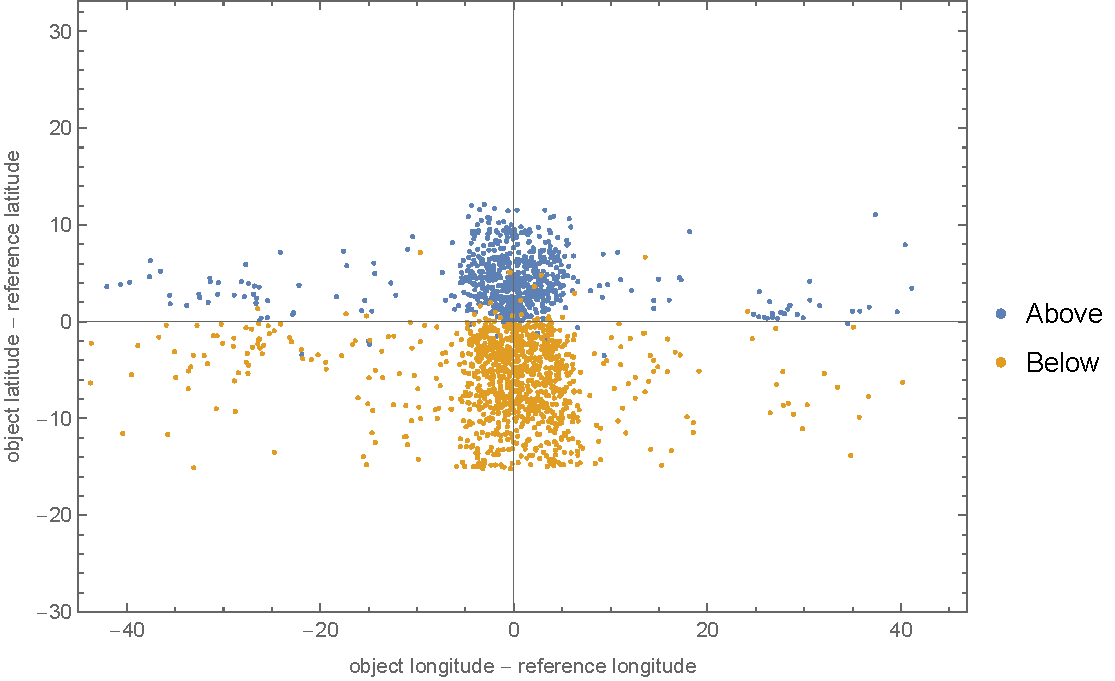
\includegraphics[width=0.7\linewidth]{aboveBelowScatter.pdf}
    \caption{Relative positions of objects and references in observations where the relation was ``above'' or ``below'' at midnight UTC+3.}
    \label{fig:scatterAboveBelow}
\end{figure}

Doing the same for observations that are ``in front of'' or ``behind'' a reference shows that objects that are ``in front of'' a reference have lower ecliptic longitude, while those that are ``behind'' have higher ecliptic longitude (figure \ref{fig:scatterInFrontOfBehind}).

\begin{figure}[h]
    \centering
    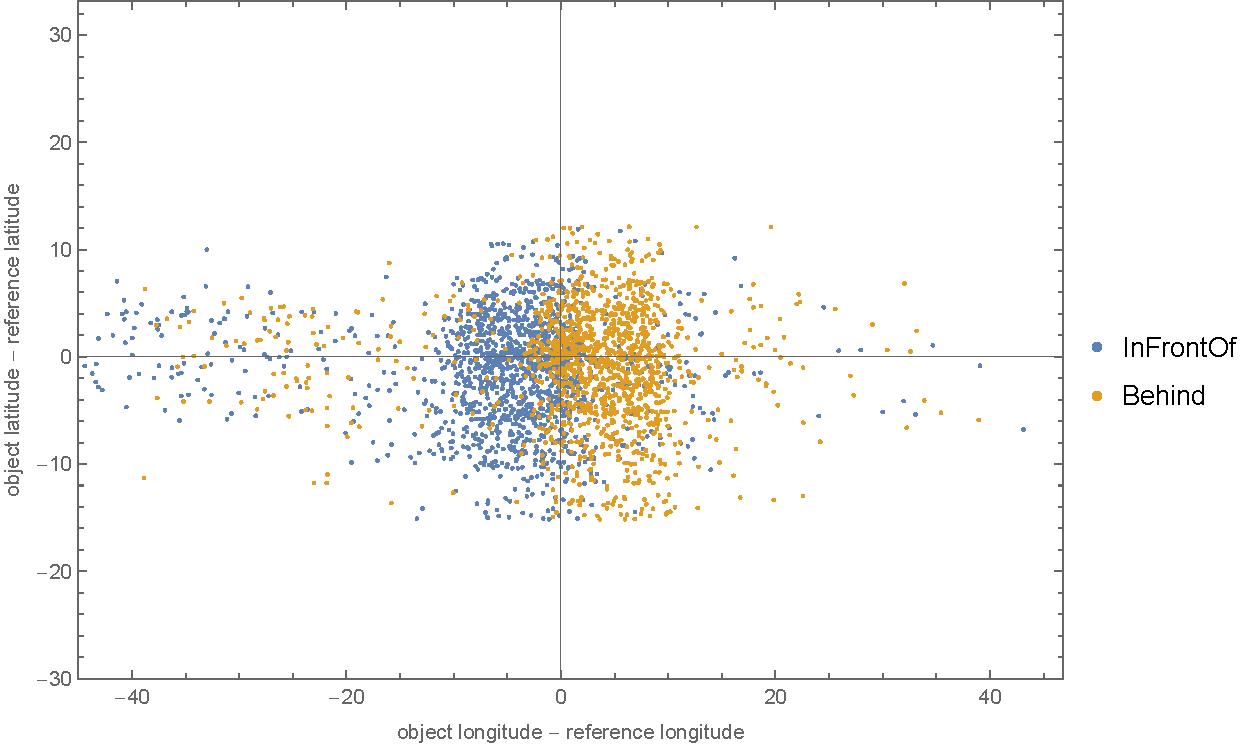
\includegraphics[width=0.7\linewidth]{infrontofBehindScatter.pdf}
    \caption{Relative positions of objects and references in observations where the relation was ``in front of'' or ``behind'' at midnight UTC+3.}
    \label{fig:scatterInFrontOfBehind}
\end{figure}

Unlike with the ``above'' and ``below'' observations, the separation between ``in front of'' and ``behind'' observations is pretty blurry. This is likely because objects generally move faster in ecliptic longitude than in ecliptic latitude, and that most ``in front of''/``behind'' observations are of the Moon (which moves faster than the planets), so the simplification that all observations occurred at midnight begins to break down.

However, the Babylonians helpfully told us when they made observations, or at least if they were at ``the first part of the night'', ``the beginning of the night'', ``the middle part of the night'', or ``the last part of the night''. This motivated the creation of a statistical model for estimating the times when observations were made, and for estimating the length of a cubit along the way.

\section{Bayesian Model}
In addition to uncertainty about the times when observations were made, there is also uncertainty about the length of a cubit. In mathematical texts, a cubit is taken to equal $2^\circ$\autocite{sachsHunger}. However, previous work has estimated that the measured cubits in the Astronomical Diaries are closer to $2.27^\circ$\autocite{jones}.

As an application of this dataset, I fit a Bayesian model to all distance observations in the Astronomical Diaries to simultaneously estimate observation times and the length of a cubit.

(I had a version of this model that simultaneously tries to estimate the length of a finger, to further check if there are 24 or 30 fingers in a cubit. However, that model had some issues, so for now I assume that there are 24 fingers in a cubit.)

The model is briefly described below.

\subsection{Variables OLD}
\begin{align*}
    c_i &: \text{observed distance in observation $i$ (in cubits)} \\
    t_i &: \text{observed time category of observation $i$} \\
    l_c &: \text{length of a cubit (in degrees)} \\
    % \epsilon &: \text{$y$-intercept (in degrees)} \\
    \sigma_y &: \text{observation variance} \\
    \mu_\text{outlier} &: \text{mean cubits for outlier observations} \\
    \sigma_\text{outlier} &: \text{variance of cubits for outlier observations} \\
    o_t &: \text{time in hours relative to midnight (UTC+3) when observations in category $t$ were made} \\
    X_i(\tau) &: \text{true distance in degrees for observation $i$ at time $\tau$ (computed with JPL ephemerides)} \\
    p &: \text{proportion of observations that are outliers} \\
    m_i &: \text{whether an observation $i$ is an outlier}
\end{align*}

\subsection{Variables}
\begin{align*}
    c_i &: \text{observed distance in observation $i$ (in cubits)} \\
    l &: \text{length of a cubit (in degrees)} \\
    \sigma &: \text{observation variance} \\
    \delta_i^\star &: \text{true distance in degrees for observation $i$ at time $\tau$ (computed with JPL ephemerides)}
\end{align*}

\subsection{Model}
\begin{align*}
    l &\sim \textrm{Normal}_{+}(2,1) \\
    \sigma &\sim \textrm{Gamma}(1/2,1/2) \\
    \mathbf{\Pi}^\textrm{(obj)} &\sim \textrm{Dirichlet}(1,1,\dots) \\
    \mathbf{\Pi}^\textrm{(ref)} &\sim \textrm{Dirichlet}(1,1,\dots) \\
    \mathbf{\Pi}^\textrm{(axis)} &\sim \textrm{Dirichlet}(1,1) \\
    Z^\textrm{(obj)}_i &\sim \textrm{Categorical}(\mathbf{\Pi}^\textrm{(obj)}) \\
    Z^\textrm{(ref)}_i &\sim \textrm{Categorical}(\mathbf{\Pi}^\textrm{(ref)}) \\
    Z^\textrm{(axis)}_i &\sim \textrm{Categorical}(\mathbf{\Pi}^\textrm{(axis)}) \\
    \Delta d_i &\sim \textrm{BetaBinomial}(1/2,1/2,d^\textrm{(min)}_i-d^\textrm{(max)}_i) \\
    d_i &= d^\textrm{(min)}_i + \Delta d_i \\
    \delta^\star_i &= \delta(Z^\textrm{(obj)}_i,Z^\textrm{(ref)}_i,Z^\textrm{(axis)}_i,d_i) \\
    c_i &\sim \textrm{Normal}(\delta^\star_i / l, \sigma)
\end{align*}

\subsection{Model}
\begin{align*}
    \textrm{cubitlength} &\sim \textrm{Normal}_{+}(2,1) \\
    \textrm{distancevariance} &\sim \textrm{Gamma}(1/2,1/2) \\
    \textrm{objectdist} &\sim \textrm{Dirichlet}(1,1,\dots) \\
    \textrm{referencedist} &\sim \textrm{Dirichlet}(1,1,\dots) \\
    \textrm{axisdist} &\sim \textrm{Dirichlet}(1,1) \\
    \textrm{object}_i &\sim \textrm{Categorical}(\textrm{objectdist}) \\
    \textrm{reference}_i &\sim \textrm{Categorical}(\textrm{referencedist}) \\
    \textrm{axis}_i &\sim \textrm{Categorical}(\textrm{axisdist}) \\
    \textrm{dateoffset}_i &\sim \textrm{BetaBinomial}(1/2,1/2,\textrm{earliestdate}_i-\textrm{latestdate}_i) \\
    \textrm{date}_i &= \textrm{earliestdate}_i + \textrm{dateoffset}_i \\
    \textrm{truedistance}_i &= \textrm{computetruedistance}(\textrm{object}_i,\textrm{reference}_i,\textrm{axis}_i,\textrm{date}_i) \\
    \textrm{cubits}_i &\sim \textrm{Normal}(\textrm{truedistance}_i / \textrm{cubitlength}, \textrm{distancevariance})
\end{align*}

\subsection{Results}
The model was fit with Markov chain Monte Carlo (MCMC).

\subsubsection{Length of a Cubit}
The cubit was estimated to be about $2.4^\circ$ (figure \ref{fig:lengthOfCubit}), which is similar to what others have found.

\begin{figure}[h]
    \centering
    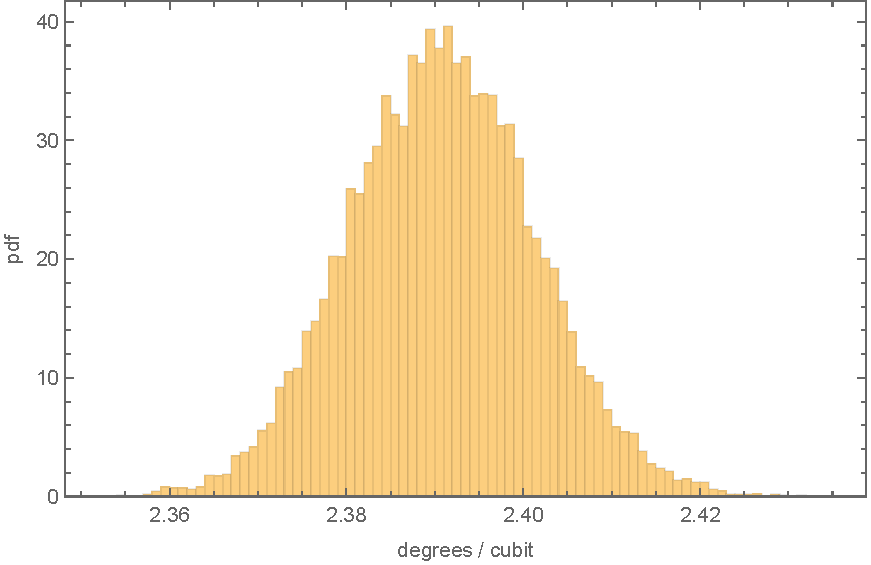
\includegraphics[width=0.6\linewidth]{lengthOfCubit.pdf}
    \caption{Estimate of the length of a cubit. Mean of $2.39^\circ$.}
    \label{fig:lengthOfCubit}
\end{figure}

\subsubsection{Observation Times}
The model also estimates when observations in each time category (e.g. ``first part of the night'') were made relative to midnight UTC+3. It estimated that the ``beginning of the night'' corresponds approximately to sunset, and ``last part of the night'' approximately to sunrise (figure \ref{fig:timeEstimates}). The estimate for the ``middle part of the night'' is very uncertain because there are only a handful of distance observations made at the ``middle part of the night''. The estimate for observations where the time category was missing is more puzzling. (In the future, observations where the time category could not be determined should be split into those where the time category was written but was damaged, and those where no time category was given in the original text.)

\begin{figure}[h]
    \centering
    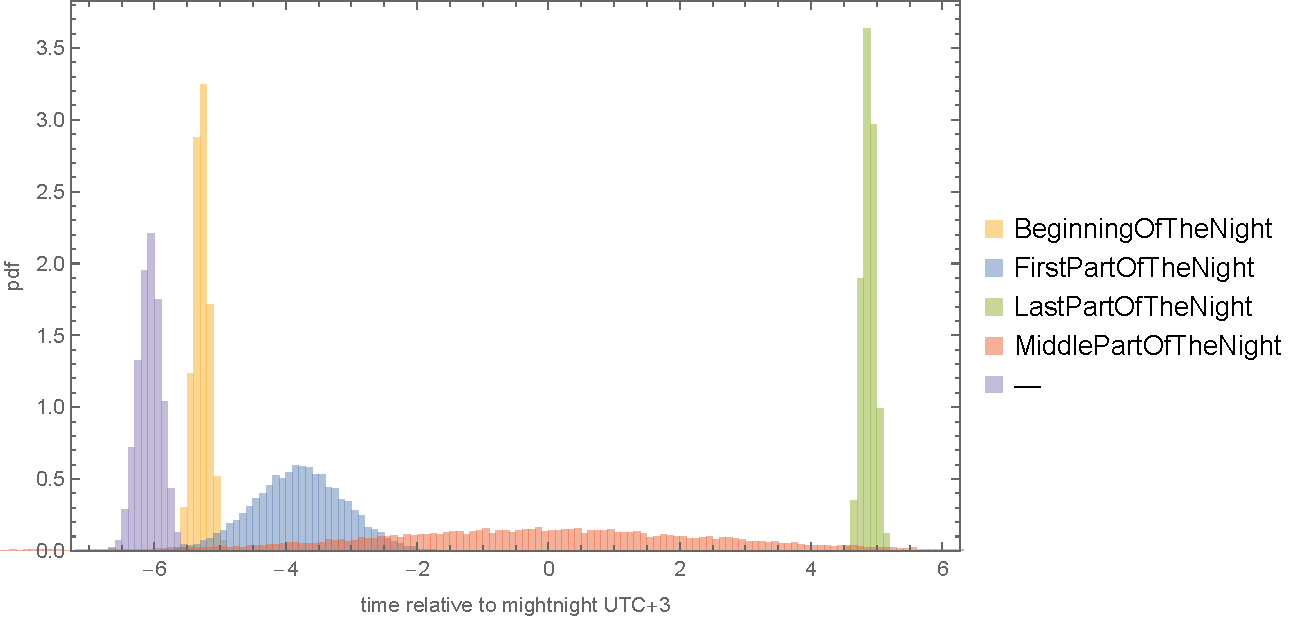
\includegraphics[width=0.75\linewidth]{timeEstimates.pdf}
    \caption{Estimates of when observations in different time categories were made. ``--'' represents observations where no time category was given, or where it could not be determined (perhaps because of damage).}
    \label{fig:timeEstimates}
\end{figure}

With these estimates of observation times, the separation between ``in front of'' and ``behind'' observations is much clearer (figure \ref{fig:scatterInFrontOfBehindTimeAdjusted}) compared with the positions at midnight (figure \ref{fig:scatterInFrontOfBehind}). This is a good sign both for the Bayesian model, and for the quality of the data.

\begin{figure}[h]
    \centering
    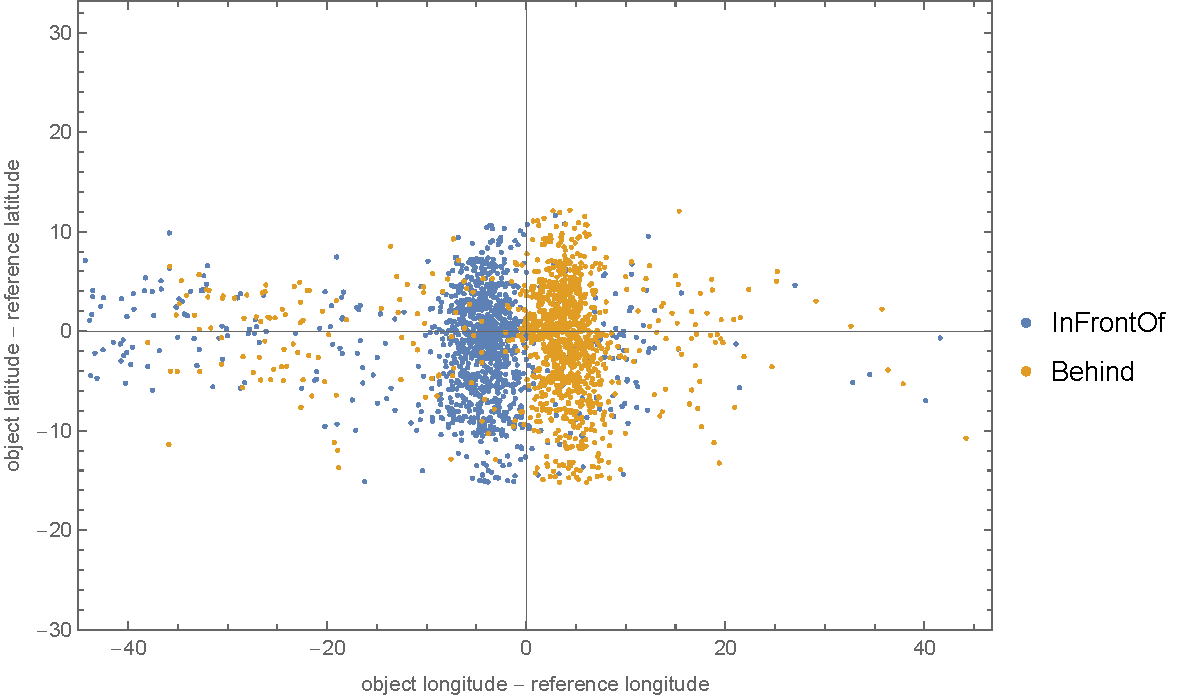
\includegraphics[width=0.7\linewidth]{infrontofBehindScatterTimeAdjusted.pdf}
    \caption{Relative positions of objects and references in observations where the relation was ``in front of'' or ``behind'' at estimated observation times.}
    \label{fig:scatterInFrontOfBehindTimeAdjusted}
\end{figure}

\subsubsection{Outliers}
The model also produces estimates of the probability that a given observation is an outlier. Outliers should include errors from the data extraction process, translation errors, errors in the Oracc versions of the texts (of which I have found a few), and ancient errors.

The model appears to have accurately identified outlier observations when fitting (figure \ref{fig:outliers}). However, I noticed that there are some patterns in what sorts of observations are outliers, which I explore below.

\begin{figure}[h]
    \centering
    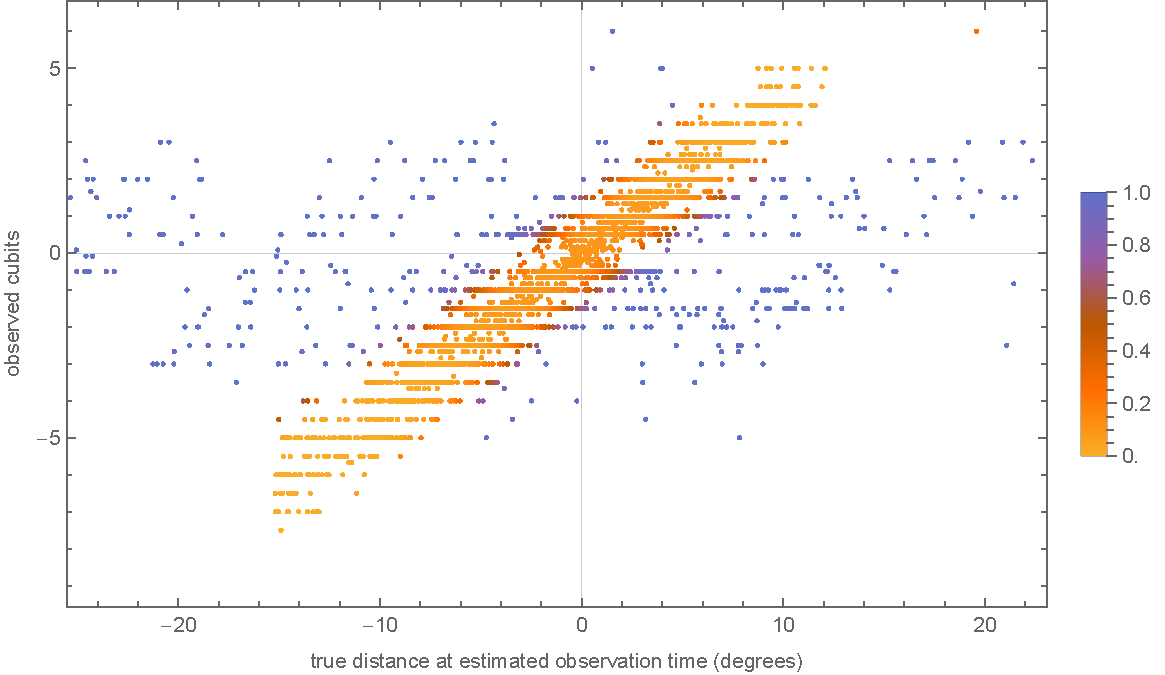
\includegraphics[width=0.7\linewidth]{outliers.pdf}
    \caption{True and observed distances between objects and references, colored to show the probability each observations is an outliers. A simplified version of the model where observation times are not estimated is essentially a linear regression on this data.}
    \label{fig:outliers}
\end{figure}

\section{Moon-Jupiter Observations}
While manually inspecting outlier observations, I found several observations of the Moon relative to Jupiter. After manually checking several, these seemed to be correctly extracted from the text, but they do not align well with the JPL ephemerides.

I looked at every pair of objects and references, and compared the number of observations made with the number of outlier observations (figure \ref{fig:outlierPairs}). For most pairs of objects, there is an approximately fixed fraction of observations that are outliers, indicating that the probability an observation is an outlier is largely independent of the objects be observed. However, the big exception is observations of the Moon relative to Jupiter, which show many more outliers that would be expected.

\begin{figure}[h]
    \centering
    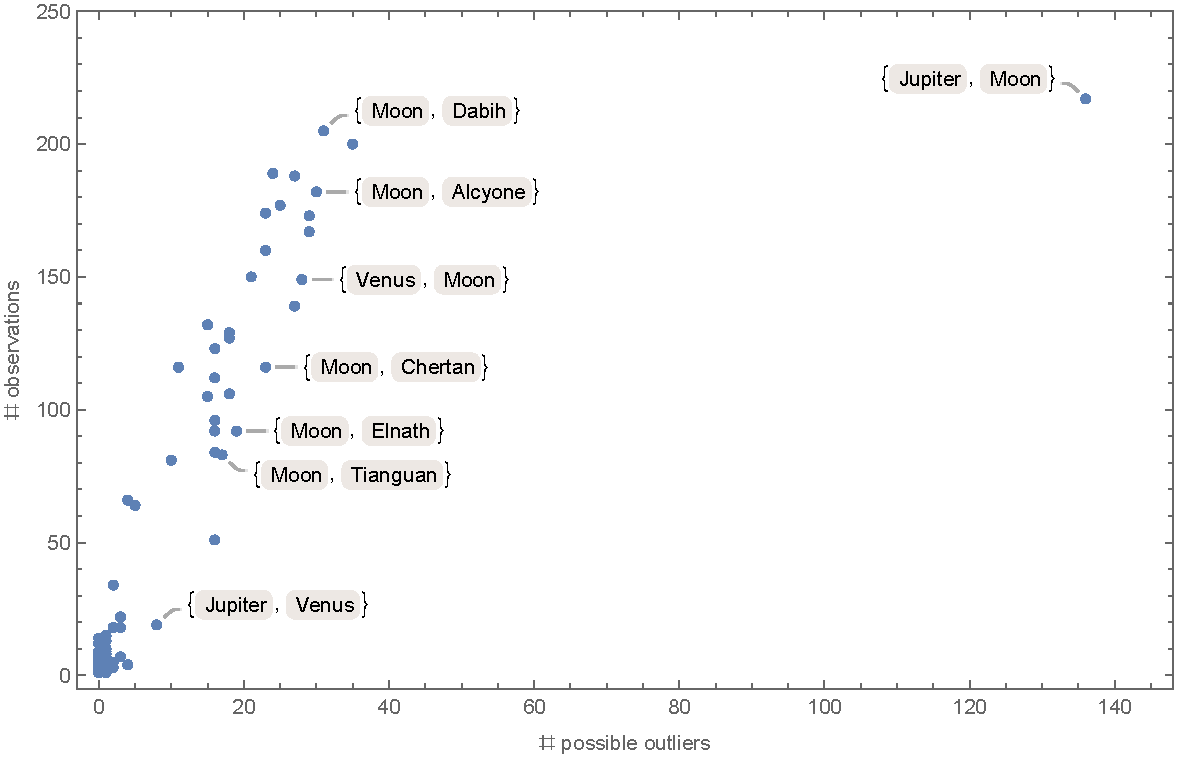
\includegraphics[width=0.6\linewidth]{outlierPairs.pdf}
    \caption{The number of observations of any pair of objects, compared with the number of outlier observations. Observations of the Moon relative to Jupiter show a much higher rate of rate of outliers.}
    \label{fig:outlierPairs}
\end{figure}

Further inspection shows that observations of the Moon being ``above'' or ``below'' Jupiter are generally accurate. However, observations of the Moon behind ``in front of'' or ``behind'' are consistently off by about $30^\circ$, a huge amount (figure \ref{fig:jupiterOutliers}). No such effect exists for any of the other planets. I don't have a good explanation of this.

\begin{figure}[h!]
    \centering
    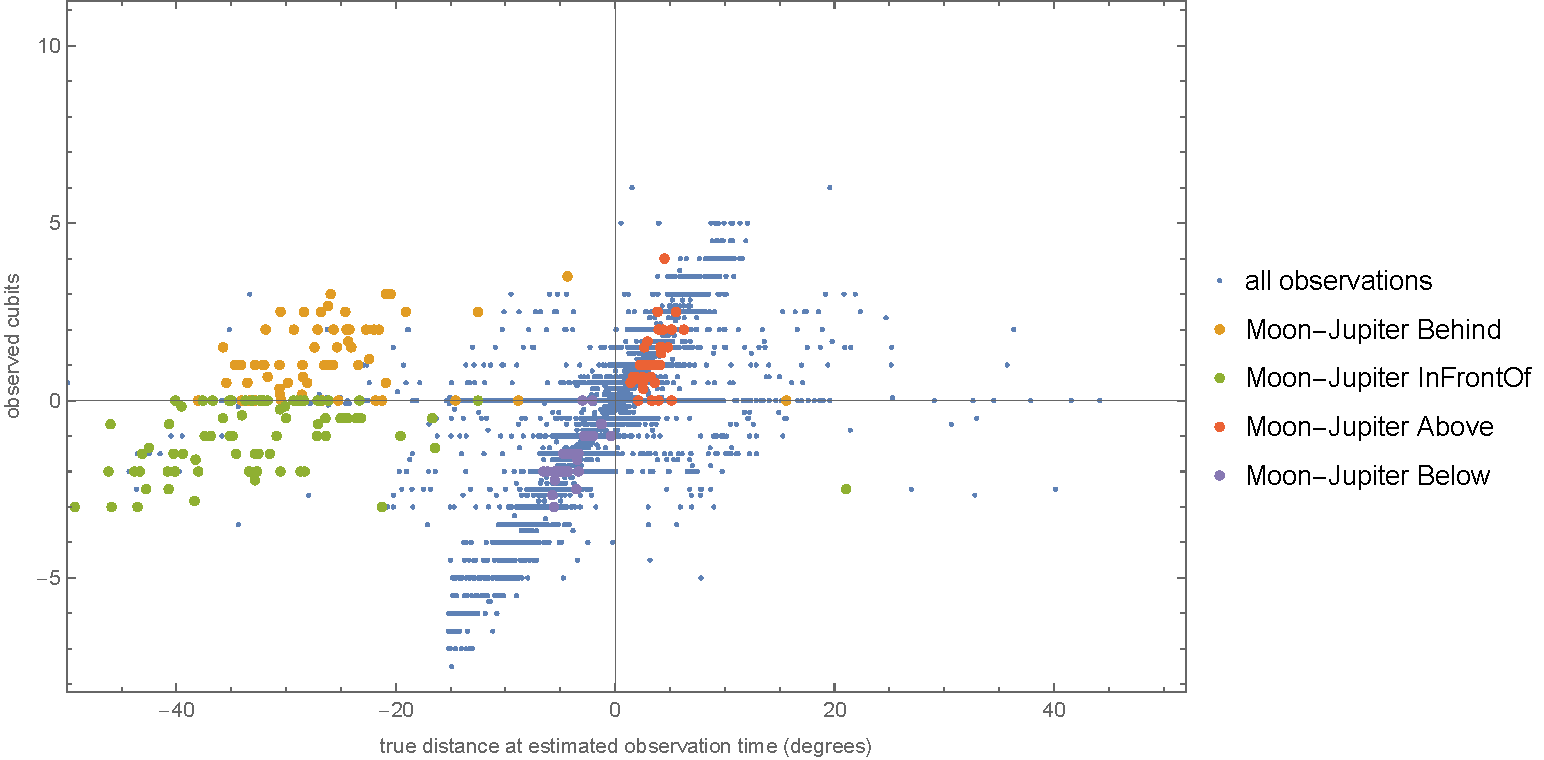
\includegraphics[width=0.8\linewidth]{jupiterOutliers.pdf}
    \caption{True vs reported distances between objects and references. There appears to be systematic errors in longitudinal observations of the Moon relative to Jupiter.}
    \label{fig:jupiterOutliers}
\end{figure}

\section{Validation}
There is still more work to be done in assessing the quality of the dataset. So far, I've used a few strategies for validation.

First, I sampled several random tablets from the data, and checked by hand whether the LLM extracted the data correctly. So far, this has revealed very few errors.

Next, I looked at outliers in some of the analysis above. This revealed a few errors that came from misidentifying the month when an observation was made. (However, this was not the case for the Moon-Jupiter observations.)

Finally, I've compared this dataset to the planetary observations collected by Alexander Jones \autocite{jones}. There is some more systematic work to be done, but so far there appears to be pretty good alignment between the two.

There are some remaining validation strategies that I also haven't implemented yet. For example, I should compare this dataset to the texts that I manually curated back in 2020.

\section{Next Steps}
There are a few next steps:
\begin{itemize}
    \item Do more validation, particularly by comparing to existing datasets (for example, from Alexander Jones, or from my manually curated data.)
    \item Add an addition LLM pass to double-check observations, and to tag fragmentary or ambiguous ones.
    \item I think the Bayesian model may be indicating higher certainty that it should by assigning most of the variance to $\sigma_y$ (observational error), as opposed to uncertainty in the length of a cubit or in observation times. More experimentation is needed to test this.
    \item Add support for more observation types. Of particular interest are the zodiacal observations (where a planet is observed to be in a sign of the zodiac), as well as weather.
\end{itemize}

\medskip

\printbibliography

\section{Appendix: Prompts}
All prompts below use few-shot learning, which involves giving a description of the task along with examples demonstrating how to perform the task correctly. The prompts below only show the instructions, but they are always followed by examples of ideal inputs and outputs.

\subsection{Line-Month Alignment}
\begin{lstlisting}
Below is an ancient Babylonian text containing astronomical observations. For each line in the text, identify the month and year that the line covers, and return the result in a JSON format.

## Instructions
1. **Determine the Year**
	- If a section starts with the year, use that year for all observations in that section, or until the months wrap around.
	- Years are always written as a dynasty followed by a number. For example 'SE 30' or 'ArtII 26'.
	- If no year is explicitly stated, infer the year from the year guide.
2. **Determine the Month**
	- The text is broken into sections shown with multiple line breaks.
	- A new section can also be indicated by going form the obverse to the reverse of the tablet, as indicated by the line number switching from something like 'o 10' to something like 'r 1'.
	- For every in the text line, identify which month is discussed in that line.
	- Allowed months are I, II, III, IV, V, VI, VI2, VII, VIII, IX, X, XI, XII, XII2. Only write months in the allowed format.
	- If a section starts with the month, use that month for all observations in that section.
	- If no month is explicitly stated, refer to the month guide to infer the order of months. The month guide will look something like '[I] II III [ ] VII-X ['.
		+ Each roman numeral in the month guide corresponds to a section of the text in order.
		+ Bracked roman numerals like '[I]' represent that a month was written, but it has been destroyed, and no longer appears in the surviving text.
		+ Empty brackets like '[ ]' mean that the intervening months are missing, or that there are sections in the text that could not be dated.
		+ Hyphenated guides like 'VII-X' mean that all the months from VII to X appear in order.
	- Every month is represented in the month guide. Only assign months to lines if those months are represented in the month guide.
	- If the month is ambiguous, or if the month guide says something like '...' or '[...]' or '[ ]' for that section, write null in the month JSON field.
3. **Missing or Ambiguous Data**
	- If the month is missing or ambiguous, write 'null' in the month JSON field. For example, `{'"line":"o 3","month":null,"year":"SE 30"}`
4. **Edges**
	- Lines marked b.e. or l.e. represent writing on the bottom edge of the text. This is like the binding of the book, so it might contain information about what year(s) or month(s) the entire text covers.
5. Write an out your reasoning and an explaination of how you assigned lines to months. Make it consise, but explain how you determined where the months breaks are, and how they relate to the month guide.
6. **Output Format**
	- Return the results in a JSON format WITH NO LINE BREAKS.
	- Return a JSON object of the form `{'explaination':'...','results':[...]}` where the array contains an object for EVERY LINE in the input text, with the format like: `{"line":"o 3","month":"XI","year":"SE 30"}`.

## Example Input
<Example inputs and outputs>
\end{lstlisting}

\subsection{Distance Observation Extraction}
\begin{lstlisting}
Below is a translation of an ancient Babylonian tablet recording astronomical observations and other information. These records include observations of the relative positions of celestial objects such as the Moon and planets in relation to stars, expressed in terms of cubits and fingers (similar to degrees).

Your task is to extract relative position observations and convert them into a compact JSON format with minimal whitespace.

## Instructions:
1. **Extract Only Relevant Observations**: Ignore observations that do not fit the specified format.
	- Only extract relative position observations that roughly follow the format: <Object> was <c> cubits <f> fingers <Relation> <Reference>. For example, 'the Moon was 1/3 cubit 3 fingers in front of \[Alpha] Cancri'.
2. **Use Fractions for Measurements**: Maintain the use of fractions (e.g., 1/3) instead of decimal numbers.
3. ** Determine the Time
	- Allowed times are:
		+ beginning of the night
		+ first part of the night
		+ middle part of the night
		+ last part of the night
	- If no allowed time is mentioned, write null in the time field.
4. ** Determine the Relation
	- Allowed relations are:
		+ in front of
		+ behind
		+ above
		+ below
		+ north
		+ south
		+ east
		+ west
	- If no allowed relation is mentioned, write null in the relation field.
5. **Handle Missing or Ambiguous Data**: 
	- If any piece of data (e.g., distance in cubits or fingers) is missing, write null in the corresponding JSON field.
	- If the relation or reference is not clear, write null in those fields.
6. **Output Format**: Write only the JSON data. Do not include any additional text or markdown. Write compact JSON with minimal whitespace. DO NOT ADD LINE BREAKS OR TABS IN THE JSON OUTPUT.
\end{lstlisting}

\end{document}
